\documentclass[12pt]{article}
\usepackage[utf8]{inputenc}
\usepackage{amsmath}
\usepackage{graphicx}
\graphicspath{ {./include/} }
\usepackage{float}
\usepackage{hyperref}
\usepackage{xcolor}
\usepackage{listings}
\usepackage{caption}
\DeclareCaptionFont{white}{\color{white}}
\DeclareCaptionFormat{listing}{%
	\parbox{\textwidth}{\colorbox{gray}{\parbox{\textwidth}{#1#2#3}}\vskip-4pt}}
\captionsetup[lstlisting]{format=listing,labelfont=white,textfont=white}
\lstset{frame=lrb,xleftmargin=\fboxsep,xrightmargin=-\fboxsep}
\newcommand{\comment}[1]{}
%opening
\title{Radiative Corrections Framework\\ A Quick Start Guide}
\author{Fady Shaker}


\begin{document}

\maketitle
\tableofcontents
\newpage
\section{Introduction}
This document will walk you through how to use and modify the radiative corrections framework starting from creating the particle guns till producing the efficiency ratios required for a fake data study.\\

The full code is accessible at:\\
\url{https://github.com/f-shaker/radiative_correction}\\
and the generated root files for the analysis are available at:\\
\url{https://yuoffice-my.sharepoint.com/:f:/r/personal/fshaker_yorku_ca/Documents/radcorr_root_files?csf=1&web=1&e=BsrP6P}

\subsection{Framework Overview}
\begin{figure}[!ht]
	\center{
	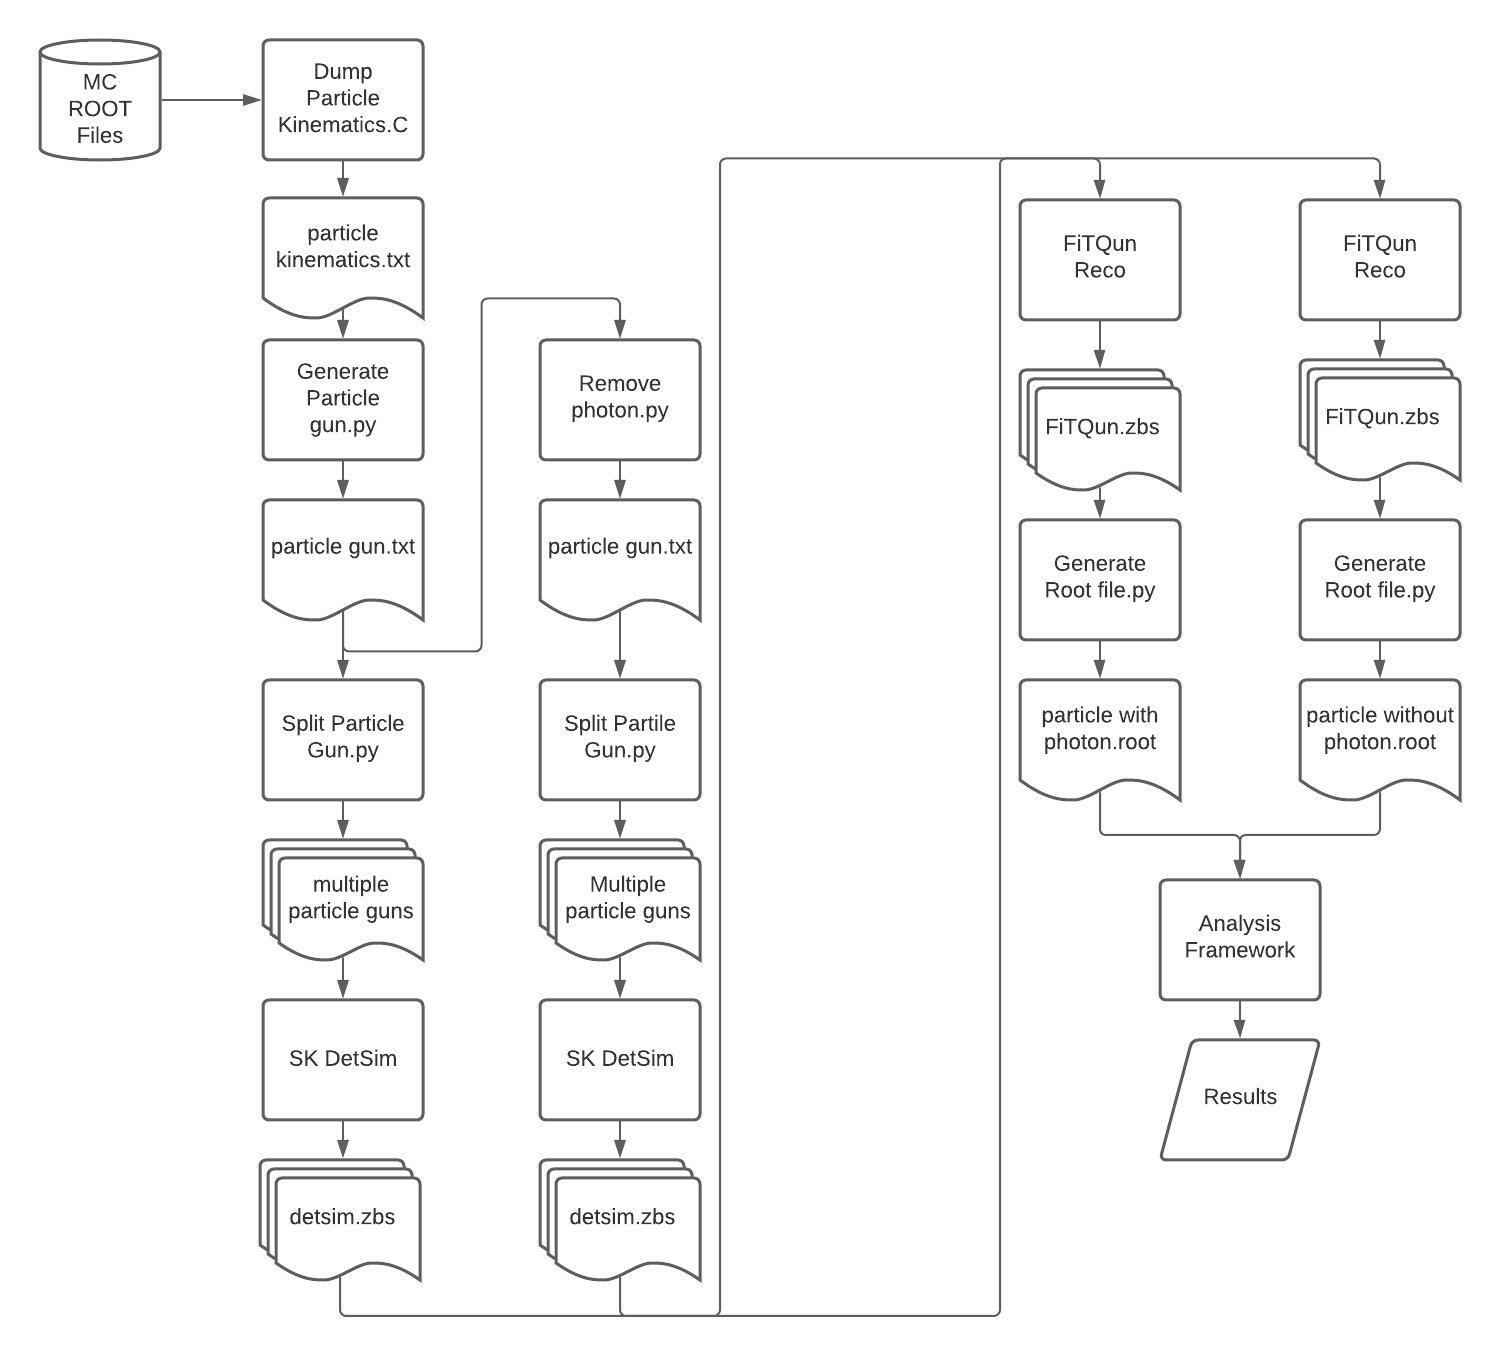
\includegraphics[scale=0.5]{radcorr_sw_framework.jpeg}
	\caption{Radiative Correction Framework}	
	}
\end{figure}
\section{Creating a Particle Gun}
\subsection{Dumping Particle Kinematics}
\label{dump_particle_kinematics}
In order to create a realistic particle gun, covering the full SK detector volume, the vertex position and output lepton ($\mu^-$, $e^-$, $\mu^+$, $e^+$) kinematics are read for the unoscillated SK MC files. This operation is done on two steps:\\
\begin{enumerate}
	\item Adding the MC files to create a single root file through hadd\\
\begin{lstlisting}[language=Python, caption=Combining MC ROOT files]
python hadd_nu.py --particle=<particle type>							
\end{lstlisting}
where $<$particle type$>$ can  be ``nue", ``nuebar", ``numu" or ``numubar" .
	\item Dump the content of the single root file into a text file containing the vertex position of a specific interaction (NEUT code) and output lepton total energy and direction. 
Change the dump\_particle\_kinematics.C configurations (e.g. input and output files). Then, from ROOT run
\begin{lstlisting}[language=C++, caption=Dumping Particle Kinematics]
dump_particle_kinematics(particle_pdg)	
\end{lstlisting}	
\end{enumerate}
At the end of this step, we will have a text file with the following format:\\
Energy dir\_x dir\_y dir\_z vertex\_x vertex\_y vertex\_z 	
\subsection{Adding the Photon}
The particle kinematics produced from the above step, does not contain any photons. Now, we will add a photon associated with that lepton at the same vertex and conserve energy, so the final output lepton energy = initial output lepton energy + photon energy.\\

 This is done by configuring the `` particle\_gun\_generator.py" script; mainly the ``MAX\_GAMMA\_EN" and the ``MAX\_GAMMA\_OPENING\_ANGLE" parameters. When the ``MAX\_GAMMA\_EN" is set to ``INFINITY" the photon maximum energy will be sampled up to the maximum available energy of the interaction, i.e the lepton energy - the lepton rest mass. Set the ``MAX\_GAMMA\_OPENING\_ANGLE" to 180, for a full $4\pi$ isotropic radiation.
Then modify the call of the main function accordingly
\begin{lstlisting}[language=Python, caption=Adding Photons ]
 def generate_radiative_corr_particle_gun(particle= 'mu-',
 nb_events=1, ip_lep_kinematics_file=None,
 file_name='pg.txt', plot_dist=False)							
\end{lstlisting}
where the ``ip\_lep\_kinematics\_file" is the text file produced from step \ref{dump_particle_kinematics} and call the script as usual
\begin{lstlisting}[language=Python, caption=Adding Photons ]
python particle_gun_generator.py							
\end{lstlisting}
\subsection{Removing the Added Photons}
This might seem a redundant step of why we shall add a photon then remove it. Well, in the analysis, we need two particle guns, one with photon and another particle gun without the photon. The output lepton kinematics in the particle gun without a photon can be equivalent to either that before emitting a photon or after emitting a photon. These two particle gun without photons scenarios are produced by calling the following script after setting the names of input and output particle gun files as well as the output lepton type 
\begin{lstlisting}[language=Python, caption=Removing Photons ]
python remove_particle_pg.py						
\end{lstlisting}
\section{SUKAP Job Submission}
This section gives some hints on how to use the framework to submit your jobs on the Japanese Cluster (SUKAP). You will need permission from the SK or the T2K-SK group to use the cluster.   
\subsection{Submitting Jobs Preparation}
The fitter, fiTQun takes few minutes per simulated event. This means that if the particle gun file was large it will exceed the maximum available walltime on SUKAP. 
Therefore, another script to divide the large particle gun into smaller files that can run within the job time limit is provided. After setting the name of the input large particle gun file, the prefix for the generated smaller particle gun file names and the maximum number of events in each small file, run  
\begin{lstlisting}[language=Python, caption=Splitting Particle Gun]
python split_particle_gun_file.py						
\end{lstlisting}
\subsection{Detector Simulation}
To run the SK detector simulation on the particle gun, edit the configuration section containing the location of the particle gun files, number of jobs to run, output location,etc. On SUKAP, run
\begin{lstlisting}[language=Python, caption=SK Detector Simulation]
python submit_radiative_skdetsim.py 						
\end{lstlisting} 
This has to be done twice: one for particle guns containing photons and one for particle guns without photons.
The output of this step is a file with a ``zbs" extension for each job.
\subsection{fiTQun}
 Then we will have to run the fitQun fitter for the output of the detector simulation. For that, you will need, as usual, to edit the configuration section of the submit\_radiative\_fitqun.py but also the fitQun data card, where all the parameters of fiTQun are presents (e.g. multiring fitting, multiple scattering, fitting hypotheses, etc.). Then on SUKAP run 
 \begin{lstlisting}[language=Python, caption=Running fiTQun]
 python submit_radiative_fitqun.py 						
 \end{lstlisting} 
 The output of this step is a file with a ``zbs" extension for each job.
 \subsection{Generating Root Files}
 We can combine the ``zbs" files output from fiTQun to create a single root file (one with photon and one without photon) using the following script (after editing the configuration section)
  \begin{lstlisting}[language=Python, caption=Generating ROOT Files]
 python generate_root.py 						
 \end{lstlisting} 
 This script will internally call the ``fillnt" script that will transform the ``zbs" files into ``hbk" then will call the ``h2root" program to convert it to a ROOT file.
  
\section{ROOT Analysis}
This section is not a complete guide for the analysis code but just give an idea on how to use some important functionalities. For more details please refer to the code itself.
\subsection{Creating the Weight Branches}
The main idea is to merge the two root files: lepton kinematics with photons (radiative) and lepton kinematics without photon (non-radiative) to produce a realistic particle gun. The created mixed-weighted root file must, at least, has a new branch that indicate if this event is radiative or not. It can also calculate the correct radiative (non-radiative) weight as well as the oscillation probabilities. However this functionality is currently overwritten in the main code.
To produce the mixed weight files, use the following function 
\begin{lstlisting}[language=C++, caption=Creating Weight Branch Example]
/*void create_weight_branches(std::string in_file_name,
bool is_sim_gamma,
fq_particle i_particle,
bool is_antiparticle)
*/
create_weight_branches("muplus_ginft180_5e4.root",
true, MUON, true);
create_weight_branches("muplus_init_5e4.root",
false, MUON, true);
/* then use hadd -f muplus_g_weighted.root
muplus_ginft180_5e4.root muplus_init_5e4.root */							
\end{lstlisting} 

\subsection{Modifying Event Weights}
Each event has a weight depending on its oscillation probability and radiative probability. This is calculated through the following function
\begin{lstlisting}[language=C++, caption= Calculating Event Weight]
/*double calculate_event_weight(bool is_mixed_weighted,
bool is_sim_gamma, t2k_sk_radiative& ana_struct,
fq_particle i_particle);
*/						
\end{lstlisting}

where the ``is\_mixed\_weighted" identify if the input file contain a mixture of weighted radiative and non-radiative events or not, the ``is\_sim\_gamma" is true if the file contains a photon, the ``ana\_struct" is a struct that is filled with all the necessary event information for the analysis, and the ``i\_particle" defines the particle type (MUON or ELECTRON).
This function will internally call the oscillation and radiative weight calculations accordingly.  

\subsection{Generating Correction Factors}
Correction factors as a function of neutrino and output lepton energies is calculated with the following functions
\begin{lstlisting}[language=C++, caption= Generating Correction Factors]
// for ccnumu and ccnumubar use
/*void check_ccnumu_event_loss_due_to_radiation3(
std::string mix_file,
std::string op_file_name)
*/
// for ccnue and ccnuebar use
/*void check_ccnue_event_loss_due_to_radiation3(
std::string mix_file,
std::string op_file_name)
*/
\end{lstlisting}
where the ``mix\_file" is the mixed weighted root file (containing both radiative and non-radiative events), and the ``op\_file\_name" is an outut file to save the generated histograms. 
\subsection{Migration from $cc\nu_\mu$ to 1e1de Sample}
To check the migration from the $cc\nu_\mu$ to 1e1de Sample call
\begin{lstlisting}[language=C++, caption= Migration Check]
// for ccnumu and ccnumubar use
/*void check_migration(std::string ip_file_name)
*/
\end{lstlisting}
passing the mixed weighted $cc\nu_\mu$ root file.
\comment{
\begin{thebibliography}{9}
	\bibitem{Ko_phd} 
	Konosuke Iwamoto. 
	\textit{Neutrino Oscillation Measurements with An Expanded Electron Neutrino Appearance Sample in T2K, 2017.}
	
	\bibitem{Kevin_talk1} 
	Kevin McFarland and Konosuke Iwamoto.
	\textit{Radiative CCQE and T2k's Oscillation Analyses, 2018}
	
	\bibitem{Rujula_calc}
	A. De Rujula, R. Petronzio and A. Savoy-Navarro
	\textit{Radiative Corrections to High-Energy Neutrino Scattering. Nucl.Phys. B154 (1979) 394. CERN-TH-2593.}
	
\end{thebibliography}
}	
\end{document}

